\begin{center}
    \textbf{Geração 1}
\end{center}

\begin{figure}[h]
    \centering
    \label{fig:geracao01}
    
    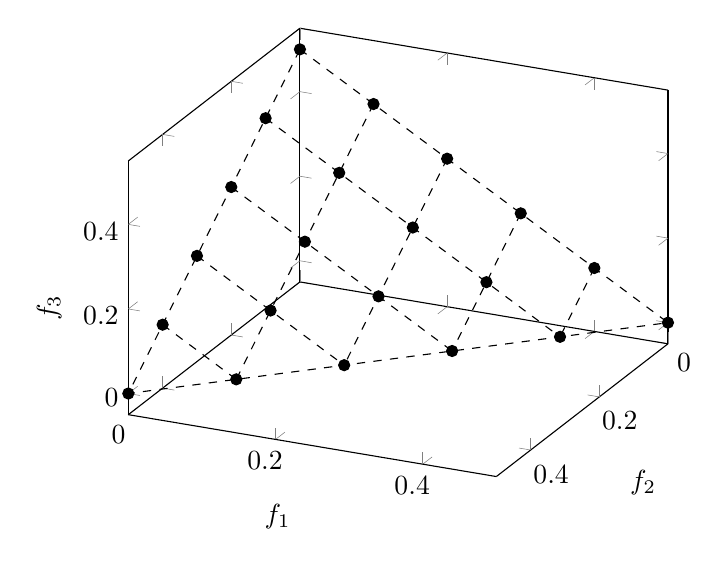
\begin{tikzpicture}[scale=1.0]
    	\begin{axis}[xlabel=$f_2$,ylabel=$f_1$,zlabel=$f_3$,view/h=115]
    		\addplot3[only marks] coordinates {
        		(0., 0., 0.5)
                (0., 0.1, 0.4)
                (0., 0.2, 0.3)
                (0., 0.3, 0.2)
                (0., 0.4, 0.1)
                
                (0., 0.5, 0.)
                (0.1, 0., 0.4)
                (0.1, 0.1, 0.3)
                (0.1, 0.2, 0.2)
                (0.1, 0.3, 0.1)
                (0.1, 0.4, 0.)
                (0.2, 0., 0.3)
                (0.2, 0.1, 0.2)
                (0.2, 0.2, 0.1)
                (0.2, 0.3, 0.)
                (0.3, 0., 0.2)
                (0.3, 0.1, 0.1)
                (0.3, 0.2, 0.)
                (0.4, 0., 0.1)
                (0.4, 0.1, 0.)
                (0.5, 0., 0.)
    		};
			\addplot3[style={dashed}]coordinates {
			    (0., 0., 0.5) (0., 0.5, 0.) (0.5, 0., 0.) (0., 0., 0.5)
			};
			
			\addplot3[style={dashed}]coordinates {(0., 0.1, 0.4) (0.4, 0.1, 0.)};
			\addplot3[style={dashed}]coordinates {(0., 0.2, 0.3) (0.3, 0.2, 0.)};
			\addplot3[style={dashed}]coordinates {(0., 0.3, 0.2) (0.2, 0.3, 0.)};
			\addplot3[style={dashed}]coordinates {(0., 0.4, 0.1) (0.1, 0.4, 0.)};
			
			\addplot3[style={dashed}]coordinates {(0.4, 0., 0.1) (0.4, 0.1, 0.)};
			\addplot3[style={dashed}]coordinates {(0.3, 0., 0.2) (0.3, 0.2, 0.)};
			\addplot3[style={dashed}]coordinates {(0.2, 0., 0.3) (0.2, 0.3, 0.)};
			\addplot3[style={dashed}]coordinates {(0.1, 0., 0.4) (0.1, 0.4, 0.)};
    	\end{axis}
	\end{tikzpicture}
    
\end{figure}

